% !TEX root = main.tex

\section{Symbolic execution of binary code}

The importance of performing symbolic analysis of program properties on binary code is on the rise for a number of reasons. Binary code analysis is attractive as it reasons on code that will actually execute: not requiring the source code significantly extends the applicability of such techniques (to, e.g., common off-the-shelf proprietary programs, firmwares for embedded systems, and malicious software), and it gives the ground truth important for security applications whereas source code analysis may yield misleading results due to compiler errors and optimizations~\cite{BITBLAZE-ICISS08}. Also, the recent advances in runtimes for programs written in dynamic languages brought just-in-time compilation to the masses, taking over on interpreters used when no efficient source-to-binary translation of code was statically possible. 

% [D] In this paragraph perhaps it is not worth mentioning obfuscation, packing and encryption
Analyzing binary code is commonly seen as a challenging task due to its complexity and lack of a high-level semantics. Modern architectures offer complex instruction sets: modeling each instruction can be difficult, especially in the presence of multiple side effects on processor flags to determine branch conditions. The second major challenge comes from the lack of the higher-level semantics present in source code, especially when no debugging information is available. Types are not explicitly encoded in binary code: even with register types, it is common to store values from one type and read them as another. Similar considerations can be made for array bounds as well. Also, control-flow graph information is not explicitly available, as control flow is performed through jump instructions at both inter- and intra-procedural level. The function abstraction at the binary level does not exist as we intend it at source-code level: functions can be separated in non-contiguous pieces, and code may also call in the middle of a code block generated for a source-level function.

In the remainder of this section we provide an overview of how symbolic executors can address some of the most significant challenges in the analysis of binary code.

\subsection{Lifting to an Intermediate Representation}
Motivated by the complexity in modeling native instructions and by the variety of architectures on which applications can be deployed (e.g., x86, x86-64, ARM, MIPS), symbolic executors for binary code typically rely on a {\em lifter} that transforms native instructions into an {\em intermediate representation} (IR, or also {\em bytecode}) as those used in compilers. The inverse process is called {\em lowering} and is performed by a compiler when it generates IR for the user-provided source code during the first step of compilation; IR is then compiled to native code for a specific platform. Source-code symbolic executors can resort to compiler-assisted lowering to reason on bytecode rather than source-language statements\mynote{[D] Java?}: for instance, \cite{KLEE-OSDI08} reasons on the IR generated by the LLVM compiler for static languages such as C and C++. Figure~\ref{fig:lowering} summarizes the relationships between source code, IR, and binary code.

\begin{figure}[h!]
  \centering
  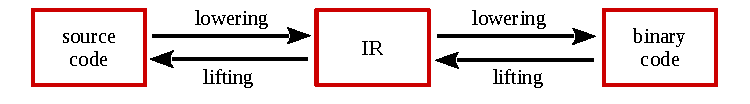
\includegraphics[width=.7\columnwidth]{images/compiler}
  \caption{\label{fig:lowering} Lowering and lifting processes in native vs. source code processing.}
\end{figure}

Reasoning at the intermediate representation level allows program analyses to be written in an architecture-independent fashion. Translated instructions will always expose all the side-effects of a native instruction, and support for additional platforms can be added over time. A number of symbolic executors use VEX, the intermediate representation format from the Valgrind dynamic instrumentation framework~\cite{VALGRIND-PLDI07}. VEX is a RISC-like language designed for program analysis that offers a compact set of instructions for expressing programs in static single assignment (SSA) form. Lifters are available for both 32-bit and 64-bit ARM, MIPS, PPC, and x86 binaries.

~\cite{ANGR-SP16} performs analysis directly on the VEX IR. Authors chose VEX over other IR formats as at that time it was the only choice that offered a publicly available implementation with support for many architectures. Also, they mention that writing a binary lifter can be a daunting task, and a well-documented and program analysis-oriented solution can be a bonus. ~\cite{BITBLAZE-ICISS08} uses VEX too, although it translates it to a custom intermediate language. The reason for this is that VEX captures the side effects of some instructions only implicitly, such as what {\tt EFLAGS} are set by x86 instructions: translating it to a custom language allowed them to simplify the development of their analysis framework.

The authors of \stwoe~\cite{CKC-TOCS12} have implemented an x86-to-LLVM-IR lifter in order to use the KLEE~\cite{KLEE-OSDI08} symbolic execution engine for whole-system symbolic analysis of binary code in a virtualized environment. The translation is transparent to both the guest operating systems and KLEE, thus enabling the analysis of binaries using the full power of KLEE. Another lifter that can be used to run KLEE on binary code is {\tt mcsema}\footnote{\url{https://github.com/trailofbits/mcsema}}.

\subsection{Reconstructing the Control Flow Graph}

\mynote{Motivate first stmt}Control flow graphs (CFGs) can provide valuable information for a symbolic executor. A fundamental issue that arises when reconstructing CFGs for binaries is that the possible targets of an indirect jump may not be identified correctly. Direct jumps are straightforward to process: as they encode their targets explicitly in the code, successor basic blocks can be identified and visited until no new edge is found. The target of an indirect jump is determined instead at run time: it might be computed by carrying out a calculation (e.g., a jump table) or depend on the current calling context (e.g., a function pointer is passed as argument, or a virtual C++ method is invoked). %We refer the interested reader to ~\cite{ANGR-SP16} for a detailed overview.

% [D] we are focusing on CFG reconstruction here rather than on its applications
% In general, not all the analyses based on CFGs require successor nodes to be accurately identified. This property can be exploited to perform further refinements on an initially less accurate CFG using techniques such as Value Set Analysis (VSA)~\cite{VSA-CC04}, which require an input CFG themselves. 
CFG recovery is typically an iterative refinement process based on a number of program analysis techniques. For instance, Value Set Analysis (VSA)~\cite{VSA-CC04} is a technique that can be used to identify a tight over-approximation of certain program state properties (e.g., the set of possible targets of an indirect jump or a memory write). In~\cite{BITBLAZE-ICISS08} an initial CFG is generated by inserting special successor nodes for unresolved indirect jump targets. This choice is conceptually similar to widening a fact to the bottom of a lattice in a data-flow analysis. When an analysis requires more precise information, VSA is then applied on demand. %Indeed, not all the CFG-based analyses require successor nodes to be accurately identified.

~\cite{ANGR-SP16} implements two algorithms for CFG recovery. An iterative algorithm starts from the entry point of the program and interleaves a number of techniques to achieve speed and completeness, including VSA, inter-procedural backward program slicing, and symbolic execution of blocks. This algorithm is however rather slow and may miss code portions reachable only through unresolved jump targets. The authors thus devise a fast secondary algorithm that uses a number of heuristics to identify functions based on prologue signatures, and performs simple analyses (e.g., a lightweight alias analysis) to solve a number of indirect jumps. The algorithm is context-insensitive, so it can be used to quickly recover a CFG without a concern for understanding the reachability of functions from one another. 

\subsection{Code Obfuscation}
In recent years, code obfuscation has received considerable attention as a cheap way to hinder the understanding of the inner workings of a proprietary program. Obfuscation is employed not only to thwart software piracy and improve software security, but also to avoid detection and resist analysis for malicious software~\cite{UDM-WCRE15,YJW-SSP15}.

A significant motivation behind using symbolic/concolic execution in malware analysis is to get around code obfuscations. However, current analysis techniques have trouble dealing with some of those obfuscations, leading to imprecision and/or excessive resource usage~\cite{YD-CCS15}. For instance, obfuscation tools can transform conditional branches into indirect jumps that symbolic analysis find difficult to analyze, while run-time code self-modification might conceal conditional jumps on symbolic values so that they are missed by the analysis.

A few works have described obfuscation techniques aiming at thwarting symbolic execution. \cite{SLG-NDSS08} introduces a {\em conditional code obfuscation} scheme based on one-way hash functions that make it hard to identify the values of symbolic variables for which branch conditions are satisfied. They also present an encryption scheme for the code to execute based on a key derived from the value that satisfies a branch condition. %Although this approach has a few limitations (for instance, it can be applied to equality tests only, and is easy to detect), it represents the first work aiming at defeating symbolic execution-based malware analyzers.
\cite{WMJ-ESORICS11} takes a step forward by proposing an obfuscation technique that makes use of linear operations only, which symbolic execution is believed to be good at analyzing. %In particular, the authors take advantage of the limitations of symbolic execution in analyzing loops:
The obfuscation tool inserts a simple loop incorporating an unsolved mathematical conjecture that converges to a known value after a number of iterations, and the produced result is then combined with the original branch condition. %Conjectures are chosen in a way that a symbolic engine would not have to discard the generated constraints for their complexity (e.g., no floating-point or non-linear operations are performed).

\cite{HOT-FPS15} presents BE-PUM, a tool to generate a precise CFG in the presence of obfuscation techniques that are common in the malware domain, including indirect jumps, structured exception handlers (SEHs), overlapping instructions, and self-modifying code. While engines such as ~\cite{BITBLAZE-ICISS08} typically rely on existing disassemblers like IDA Pro for obfuscated code, BE-PUM relies on concolic execution for deobfuscation, using a binary emulator for the user process and stubs for API calls.

\cite{YD-CCS15} discuss the limitations of symbolic execution in the presence of three generic obfuscation techniques: (1) conditional-to-indirect jump transformation, also known as {\em symbolic jump problem}~\cite{SAB-SP10}; (2) conditional-to-conditional jump transformation, where the predicate is deeply changed; and (3) symbolic code, when code modification is carried out using an input-derived value. The authors show how resorting to bit-level taint analysis and architecture-aware constraint generation can allow symbolic execution to circumvent such obfuscations.